\documentclass[12pt,a4paper]{article}
\usepackage[utf8]{inputenc}
\usepackage[german]{babel}
\usepackage[T1]{fontenc}
\usepackage{amsmath}
\usepackage{amsfonts}
\usepackage{amssymb}
\usepackage{graphicx}
\usepackage[left=2.5cm,right=2.5cm,top=2cm,bottom=2cm]{geometry}
\usepackage{float}
\author{Gruppe C14 \\ Julián Häck, Martin Koytek, Lars Wenning, Erik Zimmermann}
\begin{document}
\section{z.B. Auf- und Entladung eines Kondensators, Teilversuch 4.2}
\subsection{Versuchsbeschreibung}
\subsubsection*{Aufladung}
Das Ziel dieses Versuches ist es aus dem Strom- bzw. Spannungsverlauf beim Auf- bzw. Entladen des Kondesators die Zeitkonstante
\[\tau = R \cdot C \]
der nachfolgenden Schaltung zu bestimmen.
Nach Kirschhoff gilt in diesem Fall:
\begin{align*}
U_0-U_R(t)-U_C(t)=0 \rightarrow U_0-U_C(t)=I(t) \cdot R
\end{align*}
Nach aufstellen und lösen der DGL's ergeben sich für die Aufladung die Gleichungen:
\begin{align*}
U_C(t)=U_0 \cdot (1-e^{-\frac{t}{R \cdot C}}) \hspace{2cm} I(t)=I_0 \cdot e^{-\frac{t}{R \cdot C}}
\end{align*}
Aus denen sich nun $\tau=R \cdot C$ berechnen lässt.
\subsubsection*{Entladung}
Wird der Schalter nun geschlossen liefert uns die Maschenregel:
\begin{align*}
R \cdot I(t) + U_C(t) = 0
\end{align*}
Aufstellen und Lösen der DGL ergibt dann in diesem Fall:
\begin{align*}
U_C(t)=U_0 \cdot e^{-\frac{t}{\tau}} \hspace{2cm} I(t)=-\frac{U_0}{R} \cdot e^{-\frac{t}{\tau}}
\end{align*}
\subsection{Versuchsaufbau und Durchführung}
\begin{center}
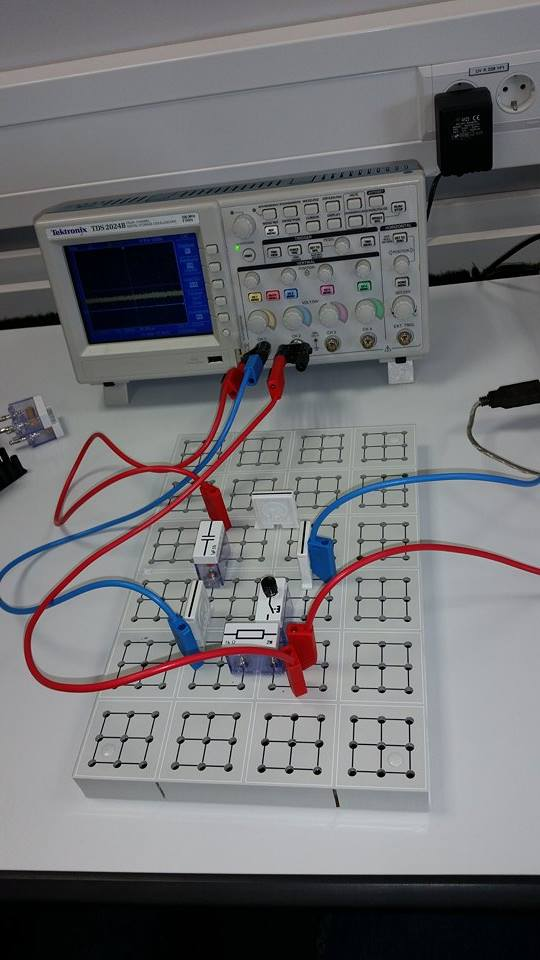
\includegraphics[scale=0.6]{12834525_1207198235971903_753892727_n.jpg}
\end{center}
Wie man im obigen Bild sieht besteht unsere Versuchsaufbau aus einem in Reihe geschalteten Kondensator und einem Widerstand. Mit dem Oszilloskop wird dann auf Channel 1 die Spannung am Kondensator und auf Channel 2 der Strom gemessen. Dafür wurde zwischen den beiden Channeln geerdet.
Die Spannungsquelle kann mittels Schalter überbrückt werden um die Entladung des Kondensators einzuleiten.
Für die Messungen wurden jeweils 1000 Werte in einem Messzeitraum von 10$ms$ aufgezeichnet. Der Messbereich der Spannung lag zwischen $-10V$ und $+10V$, die des Stroms zwischen $-0,1A$ und $+0,1A$.
Der Trigger des Oszilloskop wurde für die Aufladung auf $360mV$ aufsteigend, für die Entladung auf $1,76V$ absteigend eingestellt.
\subsection{Versuchsauswertung}
Nach dem zunächst aus den Daten die Offsests von $80mA$ bzw. $80mV$ korrigiert wurden, ergeben sich mit:
\begin{align*}
\frac{U_1}{U_2}=e^{-\frac{t_1-t_2}{\tau}}
\end{align*}
die Formeln:
\begin{align*}
\tau=\frac{\Delta t}{\ln{\frac{U_1}{U_2}}} \hspace{2cm}
\sigma_{\tau}=\sqrt{(\frac{\sigma_{\Delta t}}{\ln{\frac{U_1}{U_2}}})^2+(\frac{\Delta t}{U_1} \cdot \sigma_{U_1})^2+(-\frac{\Delta t}{U_2} \cdot \sigma_{U_2})^2}
\end{align*}
aus denen wir dann später die Kapazität C und dessen statistischen Fehler $\sigma_C$ bestimmen können.
Der systematische Fehler wurde durch die Korrektur des Offsets auf den systematischen Fehler auf $R$ reduziert. Dieser ergibt sich dann aus:
\begin{align*}
\frac{\sigma_{C,sys}^R}{C}=\frac{\sigma_{R,sys}}{R}
\end{align*}
\subsubsection{Rohdaten}
Mithilfe des Cursers des Oszilloskops wurden die Spannungen bzw. Ströme mit einem Abstand von $1ms$ abgelesen und ein Ablesefehler von $0,04mA$, $0,04V$ und $0,04ms$ notiert und anschließend durch $\sqrt{12}$ geteilt.
\begin{table}[H]\centering
\caption{Oszilloskop}
\begin{tabular}{c|c}
$I_1$& $I_2$\\ \hline
$0,72A$& $1,88A$\\ 
$0,8A$& $2,24A$ \\
$0,76A$& $2,12A$ \\
$0,72A$& $1,92A$ \\
\\
$U_1$& $U_2$ \\ \hline
$0,84V$& $2,48V$ \\
$0,84V$& $2,44V$ \\
$0,80V$& $2,40V$ \\
$0,89V$& $2,44V$ \\
\end{tabular} 
\end{table}
\subsubsection{Analyse/Transformation der Rohdaten}
Aus den Werten der Auf- und Entladung wurden anschließend jeweils $\tau$ und $\sigma_{\tau}$ berechnet und mithilfe von:
\begin{align*}
C=\frac{\tau}{R} \hspace{2cm} \sigma_C=\sqrt{(\frac{\sigma_{\tau}}{R})^2+(-\frac{\tau}{R^2}\cdot \sigma_R)^2}
\end{align*}
wurden dann die Kapazitäten und ihre statistischen Fehler berechnet.
Danach haben wir dann aus den Ergebnissen den gewichteten Mittelwert und dessen Fehler berechnet. Der systematische Fehler wurde dabei aus den Ergebnissen der Widerstandsmessung berechnet.
Zu guter Letzt haben wir die Einzelergebnisse mit ihren Gesammtfehlern zusammen mit unserem Mittelwert geplottet.
\begin{figure}[hbtp]
\centering
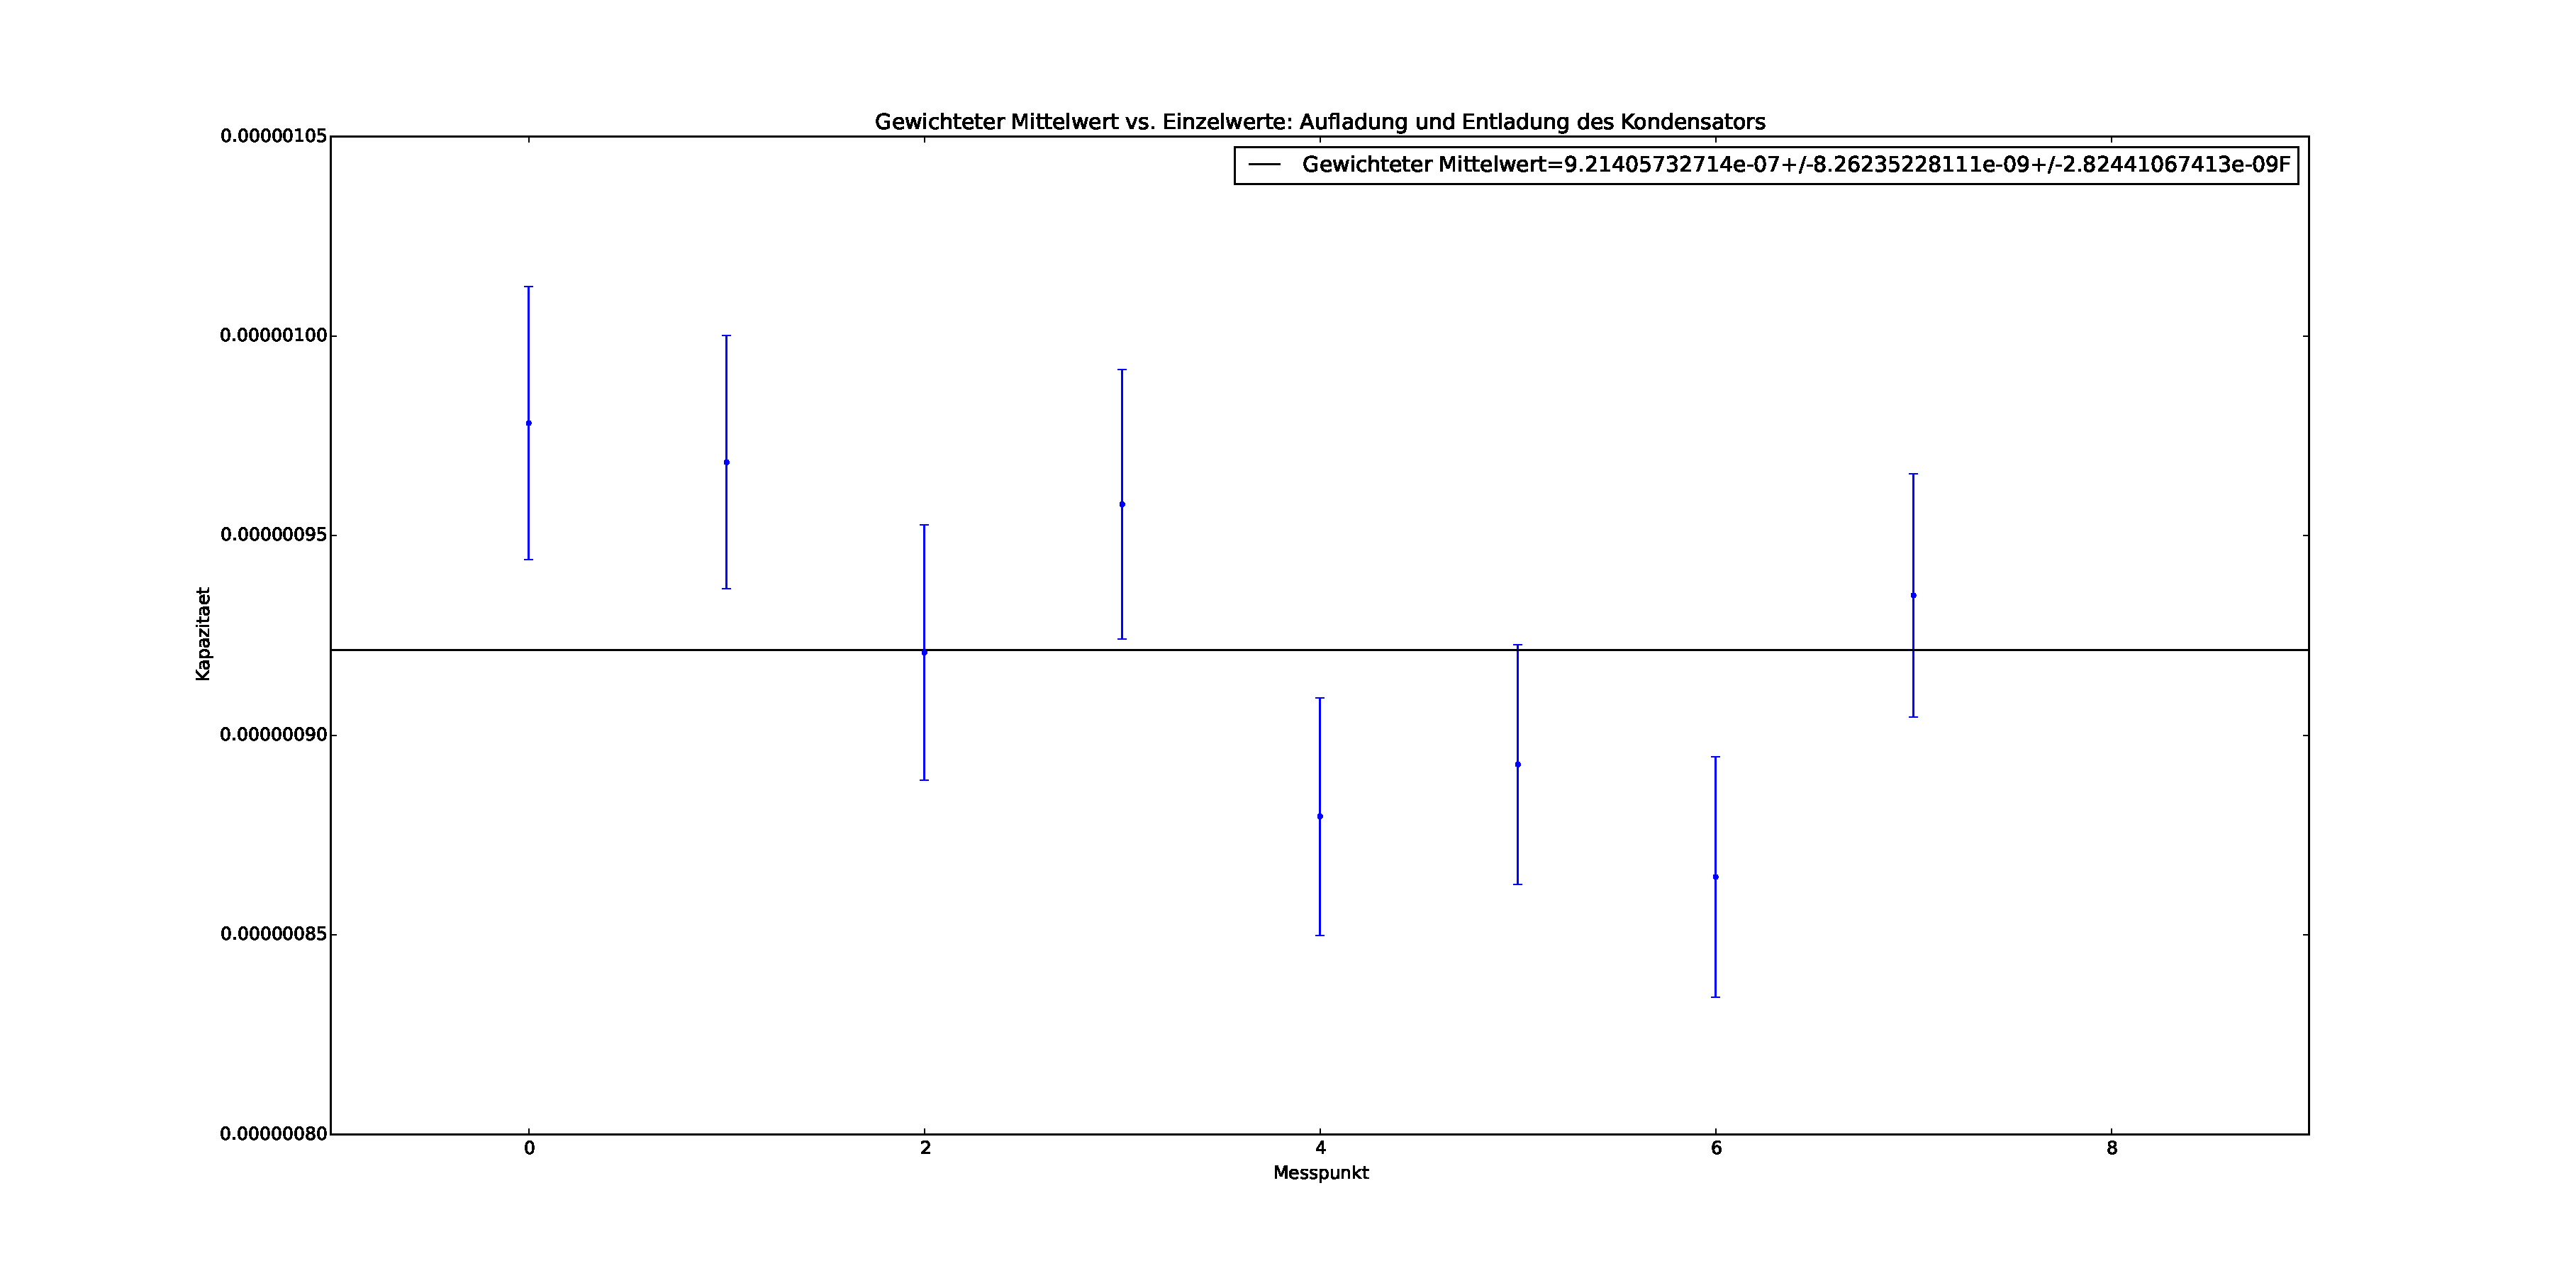
\includegraphics[scale=0.3]{auf-entladung.eps}
\caption{Ergebnisse vs. Mittelwert}
\end{figure}
\subsubsection{Fazit}
Aus den Ergebnissen der Analyse zeigt sich, dass drei der Werte für $C$ mit $1\sigma$ Abweichung und alle Werte mit $2\sigma$ Abweichung im Bereich des Mittelwerts liegen. Die etwas zu große Abweichung des Endergebnisses vom Literaturwerts von $1\mu F$ mit einer Toleranz von $5 \%$, lässt sich durch nicht berücksichtigte systematische Fehler wie z.B. ein größerer Widerstand, bedingt durch die verwendeten Kabel und Steckplattenbauteile, erklären.
\end{document}